% !TeX root =  main.tex

\chapter{Conic Sections}

\section{Parabolas}


\begin{definition}[Geometric Definition of a Parabola]

A parabola is the set of points in the plane such that the distances $|PF$ from $P$ to a fixed point $F$ (called the \textbf{focus}) and the distance $|Pl|$ from $P$ to a fixed line $l$ (called the \textbf{directrix}) are the same.

The \textbf{axis of symmetry} is the line $l_\perp$ that runs through the focus and perpendicular to the directrix. The \textbf{vertex} $V$ is the intersection of the parabola and the axis of symmetry.


The line segment that runs through the focus perpendicular to the axis, with endpoints on the parabola, is called the \textbf{latus rectum}, and its length is the \textbf{focal diameter} of the parabola.

% Because the latus rectum is parallel to the directrix and points on a parabola are equidistant from the focus and the directrix. The focal diameter equals the distance from the focus to the directrix. In particular, for a parabola with the vertex at the origin and the focus on a coordinate axis, the focal diameter is $|4p|$.
\end{definition}

% \begin{center}
%   \includegraphics[width=0.5\textwidth,keepaspectratio]{figs/parabola-concepts.png}
% \end{center}


  \begin{theorem}[Parabola with vertical axis]
  A parabola has an equation $(x-a)^2=4p(y-b)$ if and only if two of the following properties are satisfied:
  \begin{enumerate}
      \item the vertex is $V(h, k)$;
      \item the focus is $F(h, k+p)$;
      \item the directrix is $y=k-p$.
  \end{enumerate}
  
  The parabola opens upward if $p>0$ or downward if $p<0$.
  \end{theorem}
  
  \begin{theorem}[Parabola with horizontal axis]
  A parabola has an equation $(y-k)^2=4p(x-h)$ if and only if two of the following properties are satisfied:
  \begin{enumerate}
      \item the vertex is $V(h, k)$;
      \item the focus is $F(h+p, k)$;
      \item the directrix is $x=h-p$.
  \end{enumerate}
  
  The parabola opens to the right if $p>0$ or to the left if $p<0$.
  \end{theorem}


% \begin{center}
%     \includegraphics[width=0.8\textwidth,keepaspectratio]{figs/ParabolaGraphs.png}
% \end{center}
% \begin{definition}
  The equations in the above theorems are called the \textbf{standard form}.
% \end{definition}

\begin{example}
    Find an equation of the parabola with the vertex $V(0,2)$ and focus $F(4,2)$.
\end{example}

\newpage

% \begin{example}
%     Find the focus and directrix of the parabola $y=-x^2$.
% \end{example}

\begin{example}
    Find the focus, directrix, and focal diameter of the parabola $y=\frac{1}{2}x^2$.
\end{example}


\begin{example}
  Find an equation of the parabola with the focus $(1, 2)$ and the directrix $y=-2$.
\end{example}

\newpage

\begin{example}
A searchlight has a parabolic reflector that forms a “bowl,” which is 12 in. wide from rim to rim and 8 in. deep.  If the filament of the light bulb is located at the focus, how far from the vertex of the reflector is it?
\end{example}
% \vspace{-2\baselineskip}
% \begin{center}
% \noindent
% \includegraphics[height=8\baselineskip,keepaspectratio]{figs/SearchlightReflector1.png}
% \hspace{2em}
% \includegraphics[height=9\baselineskip,keepaspectratio]{figs/SearchlightReflector2.png}
% \end{center}

\begin{example}
  Find the vertex, focus, and directrix for the following parabola $3x-5=y^2-4y$.
\end{example}

\newpage

\section*{Exercises}

\begin{exercise}
  Find the vertex, focus, and directrix of the parabola. Sketch the graph.\\
  \begin{enumerate*}
      \item $x^2=-8(y-1)$.
      \item $(y+1)^2=12(x-2)$.
      \item $x^2+2x+6y=5$.
      \item $2x-y^2=2$.
  \end{enumerate*}
\end{exercise}

\begin{exercise}
  Find an equation for the conic section with the given properties.
  \begin{enumerate}
      \item The parabola with vertex at $(1,0)$ and focus $(1, 5)$.
      \item The parabola with vertex at $(2,1)$ and the directrix $x=-2$.
  \end{enumerate}
  \end{exercise}

  \newpage

\begin{exercise}
    Find an question for the conic section with the given graph.\\
\begin{tikzpicture}
  \begin{axis}[
    xmin=-2,
    xmax=2,
    ymin=-2,
    ymax=2,
    xtick={-5,-4,...,5},
    ytick={-5,-4,...,5},
    grid=major,
    enlargelimits=0.05
    ]
      \addplot[line width=1.5pt, blue, smooth, samples=100, domain=-2:2] {1/2*x^2};
      \addplot[only marks] coordinates {(0,0)(0,1/2)}; 
      \begin{pgfonlayer}{ft}
        \node at (0,1/2) [right] {Focus};
        \node at (0,0) [below left] {Vertex};
      \end{pgfonlayer}
    \end{axis}
\end{tikzpicture}
\end{exercise}
% \vspace*{-0.3\textheight}

\newpage


\section{Ellipses}

\begin{definition}[Geometric Definition of an Ellipse]
An \textbf{ellipse} is the set of points in the plane such that, for any point $P$ in it, the sum of distances $|PF_1|$ and $PF_2$ from $P$ to two fixed points $F_1$ and $F_2$ is a constant (usually denoted by $2a$). These two fixed points are the \textbf{foci} (plural of focus) of the ellipse.

The line segment through the foci with endpoints on the ellipse is called the \textbf{major axis}

The line segment perpendicular to the major axis through the center with endpoints on the ellipse is the \textbf{minor axis}.

The intersections of the ellipse and the major axis are called the \textbf{vertices} of the ellipse. The intersections of the ellipse and the minor axis are called the \textbf{co-vertices} of the ellipse.

The midpoint of foci, or vertices, or co-vertices are the same, which is called the \textbf{center} of the ellipse.

The distance of the foci to the center is called the \textbf{focal distance} or \textbf{linear eccentricity}. 

\end{definition}

\begin{proposition}
    Suppose the length of the major axis is $2a$, the length of the minor axis is $2b$, and the linear eccentricity is $c$. Then
    \[a^2=b^2+c^2.\]
\end{proposition}

\begin{theorem}[Ellipse with horizontal major axis]
An ellipse has an equation $\frac{(x-h)^2}{a^2}+\frac{(y-k)^2}{b^2}=1$ if and only if two of the following properties are satisfied:
\begin{enumerate}
  \item the foci are $(h\pm \sqrt{a^2-b^2}, k)$;
  \item the vertices are $(h\pm a, k)$;
  \item the co-vertices are $(h, k\pm b)$.
\end{enumerate}
The center of the ellipse is $(h, k)$.
\end{theorem}

\begin{theorem}[Ellipse with vertical major axis]
  An ellipse has an equation $\frac{(x-h)^2}{b^2}+\frac{(y-k)^2}{a^2}=1$ if and only if two of the following properties are satisfied:
  \begin{enumerate}
    \item the foci are $(h, k\pm \sqrt{a^2-b^2})$;
    \item the vertices are $(h, k\pm a)$;
    \item the co-vertices are $(h\pm b, k)$.
  \end{enumerate}
The center of the ellipse is $(h, k)$.
\end{theorem}

% \begin{center}
%  \includegraphics[width=0.8\textwidth,keepaspectratio]{figs/EllipseGraphs.png}
% \end{center}

The equations of ellipses in the above theorems are called the \textbf{standard form}. The ellipses 

\begin{example}
An ellipse has the equation $\dfrac{x^2}{9}+\dfrac{y^2}{4}=1$.
Find the foci, the vertices, and the lengths of the major and minor axes. Sketch the graph.
\end{example}

\newpage

\begin{example}
    Find the foci of the ellipse $16x^2+9(y-2)^2=144$.
\end{example}

\begin{example}
Find an equation of the ellipse with the vertices $(\pm 4, 1)$ and the foci $(\pm 2, 1)$.
\end{example}

\begin{definition}
The eccentricity $e$ of an ellipse is defined as
\[e=\dfrac{\text{focal distance}}{\frac12\left(\text{length of the major axis}\right)}=\dfrac{2\cdot(\text{focal distance})}{\left(\text{length of the major axis}\right)}.\]
% \begin{center}
%     \includegraphics[scale=0.8]{figs/EllipseWithVariousEccentricities.png}
% \end{center}
For an ellipse centered at the origin and with the major axis along a coordinate axis, the eccentricity is $e=\dfrac ca$.
\end{definition}


\begin{example}
    Find the equation of the ellipse with foci $(0, \pm8)$ and the eccentricity $e=\frac45$.
\end{example}


\newpage
\section*{Exercises}


\begin{exercise}
    An equation of an ellipse is given. Find the center, vertices, and foci of the ellipse, and the lengths of the major and minor axes. Sketch the graph.\\
    \begin{enumerate*}
        \item $\dfrac{x^2}{9}+\dfrac{y^2}{25}=1$.
        \item $\dfrac{(x-1)^2}{25}+\dfrac{(y+1)^2}{9}=1$.
        \item $9x^2+18x+25y^2=-8$.
        % \item $25x^2+9y^2-16=0$.
    \end{enumerate*}
\end{exercise}

\begin{exercise}
  Find an equation for the ellipse with the given properties.
  \begin{enumerate}
      \item  vertices $(\pm 2, 0)$ and foci $(\pm 1, 0)$.
      \item  foci $(1,4)$ and $(1,1)$, and the eccentricity $e=\frac34$.
  \end{enumerate}
  \end{exercise}
  
\newpage
  \begin{exercise}
      Find an question for the ellipse with the given graph.\\
      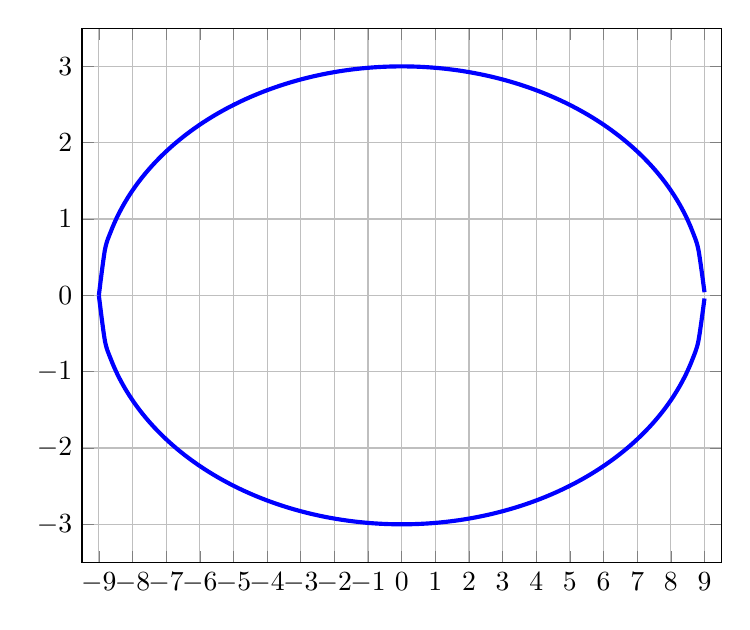
\begin{tikzpicture}
      \begin{axis}[
        width=0.8\textwidth,
        xmin=-9.5,
        xmax=9.5,
        ymin=-3.5,
        ymax=3.5,
        xtick={-10,-9,...,10},
        ytick={-5,-4,...,5},
        grid=major,
        % enlargelimits=0.5,
        ]
          \addplot[line width=1.5pt, blue, smooth, samples=100, domain=-9:9] {sqrt(9-x^2/9)};
          \addplot[line width=1.5pt, blue, smooth, samples=100, domain=-9:9] {-sqrt(9-x^2/9)};
        \end{axis}
    \end{tikzpicture}
  \end{exercise}
  % \vspace*{-0.2\textheight}

\newpage

\section{Hyperbola}

\begin{definition}[Geometric Definition of a Hyperbola]
A \textbf{hyperbola} is the set of points in the plane, such that, for any point $P$ in it, the absolute difference of the distances $|PF_1$ and $PF_2$ from $P$ to two fixed points $F_1$ and $F_2$ is a constant (usually denoted by $2a$). The fixed points $F_1$ and $F_2$ are the \textbf{foci} of the hyperbola.

The midpoint of foci is the \textbf{center} of the hyperbola.

The distance $c$ of the foci to the center is called the \textbf{focal distance} or \textbf{linear eccentricity}.

The line segment passes through the foci and ends on the hyperbola is called the \textbf{transverse axis}. 

The endpoints of the transverse axis are called the \textbf{vertices} of the hyperbola.

% The conjugate axis is the segment of length $2b$ that is perpendicular to the transverse axis and with midpoint at the hyperbola's center, where $b=\sqrt{a^2-c^2}$.

% The endpoints of the conjugate axis are called the \textbf{co-vertices} of the hyperbola.

A hyperbola consists of two separate curves, called \textbf{branches}, that are symmetric with respect to the transverse axis, conjugate axis, and center. 
\end{definition}


\begin{theorem}[Hyperbola with a horizontal transverse axis]
    A hyperbola has an equation $\frac{(x-h)^2}{a^2}-\frac{(y-k)^2}{b^2}=1$ if and only if the foci are $(h\pm \sqrt{a^2+b^2}, k)$ and the vertices are $(h\pm a, k)$.
\end{theorem}

\begin{theorem}[Hyperbola with a vertical transverse axis]
    A hyperbola has an equation $\frac{(y-k)^2}{a^2}-\frac{(x-h)^2}{b^2}=1$ if and only if the foci are $(h, k\pm \sqrt{a^2+b^2})$ and the vertices are $(h, k\pm a)$.
\end{theorem}

% \begin{center}
%  \includegraphics[width=0.8\textwidth,keepaspectratio]{figs/HyperbolaGraphs.png}
% \end{center}

% \begin{definition}
% A horizontal or oblique \textbf{asymptote} of a graph is a line with the property that the distance from the line to points on the graph approaches 0 as $x\to-\infty$ or as $x\to\infty$.
% \end{definition}

% A parabola has two asymptotes which are intersect at the center and symmetric with respect to the center or each axis.

\begin{proposition}[Characterization of hyperbola by asymptotes]
    A hyperbola centered at $(h,k)$ has an equation $\dfrac{(x-h)^2}{a^2}-\dfrac{(y-k)^2}{b^2}=r$, where $r$ is a nonzero reall number, if and only if its asymptotes are $y-k=\pm\dfrac{b}{a}(x-h)$.
\end{proposition}

\begin{definition}
  The rectangle whose diagonals are along the asymptotes and with a side containing a vertex of a hyperbola is called the \textbf{central box}.
  
  The line segment through the center, perpendicular to the transverse axis with endpoints on the central box is the \textbf{conjugate axis}.
  
  The endpoints of the conjugate axis are called the \textbf{co-vertices}.
\end{definition}

% \begin{center}
%     \includegraphics[width=0.7\textwidth,keepaspectratio]{figs/KeyConceptsOfHyperbola.jpg}
% \end{center}

\begin{example}
    A hyperbola has the equation $9x^2-16y^2=121$.
Find the vertices, foci, length of the transverse axis, and asymptotes. Sketch the graph.
\end{example}

\newpage

\begin{example}
    Find the vertices, foci, length of the transverse axis, and asymptotes of the hyperbola $x^2+2x-9y^2+10=0$. Sketch the graph.
\end{example}

\begin{example}
    Find the equation of the hyperbola with vertices $(\pm 3, 1)$ and foci $(\pm 4, 1)$.
\end{example}

\begin{example}
Find an equation of the hyperbola with vertices $(\pm 2, 1)$ and asymptotes $y=\pm\dfrac{1}{2}x+1$. 
\end{example}

\newpage
\section*{Exercises}

\begin{exercise}
    An equation of a hyperbola is given. Find the center, vertices, foci, and asymptotes of the hyperbola. Sketch the graph.\\
    \begin{enumerate*}
        \item $\dfrac{x^2}{9}-\dfrac{y^2}{25}=1$.
        \item $\dfrac{y^2}{9}-\dfrac{x^2}{25}=1$.
        \item $9x^2-25y^2=1$.
        \item $25x^2-9y^2-4=0$.
    \end{enumerate*}
\end{exercise}

\begin{exercise}
Find an equation for the conic section with the given properties.
\begin{enumerate}
    \item The hyperbola with foci $(0,\pm 3)$ and vertices $(\pm 2, 0)$.
    \item The hyperbola with foci $(\pm 5, 1)$ and asymptotes $y=\pm\frac34+1$.
\end{enumerate}
\end{exercise}

\newpage

\begin{exercise}
    Find an question for the conic section with the given graph.\\
    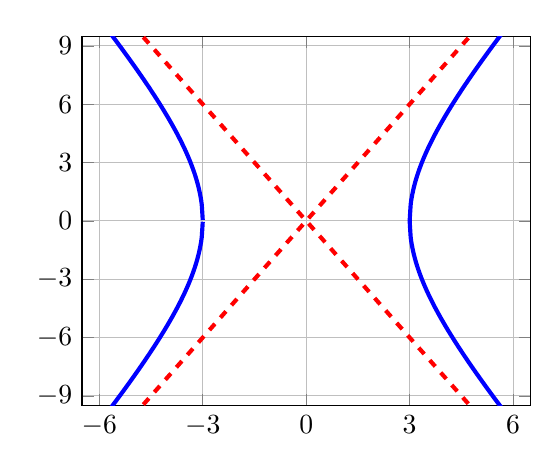
\begin{tikzpicture}
      \begin{axis}[
        width=0.6\textwidth,
        xmin=-6.5,
        xmax=6.5,
        ymin=-9.5,
        ymax=9.5,
        xtick={-9,-6,...,9},
        ytick={-9,-6,...,9},
        grid=major,
        % enlargelimits=0.5,
        ]
          \addplot[line width=1.5pt, blue, smooth, samples=100, domain=-6:-3] {sqrt(6^2*(x^2/9-1))};
          \addplot[line width=1.5pt, blue, smooth, samples=100, domain=-6:-3] {-sqrt(6^2*(x^2/9-1))};
          \addplot[line width=1.5pt, blue, smooth, samples=100, domain=3:6] {sqrt(6^2*(x^2/9-1))};
          \addplot[line width=1.5pt, blue, smooth, samples=100, domain=3:6] {-sqrt(6^2*(x^2/9-1))};
          \addplot[line width=1.5pt, red, dashed, smooth, samples=100, domain=-6:6] {2*x};
          \addplot[line width=1.5pt, red, dashed, smooth, samples=100, domain=-6:6] {-2*x};
        \end{axis}
    \end{tikzpicture}
\end{exercise}
\vspace*{-0.2\textheight}
